\subsection{Results}
We begin with our results for PFDS. These results influence our results for FVS which will be discussed subsequently. 
\paragraph{PFDS: ILP formulations and LP integrality gap.} 
We answer Question \ref{q:intro-pfds} affirmatively via a new ILP for PFDS. 
Our ILP for PFDS is based on Charikar's LP for the densest
subgraph problem (DSG) \cite{charikar_greedy_2000}. In DSG, the input is
an undirected graph $G=(V,E)$ and the goal is to find an induced subgraph $G[S]$ of
maximum density where the density of $S \subseteq V$ is defined
as ${|E(S)|}/{|S|}$. We define the density of $G$ to be $\max\{|E[S]|/|S|: \emptyset \ne S\subseteq V\}$. We note that a graph is a pseudoforest if and only if
its density is at most one. Thus, PFDS can equivalently be phrased as
the problem of finding a minimum cost subset of vertices to delete so
that the remaining graph has density at most one.  Charikar formulated
an LP to compute the density of a graph. The dual of Charikar's LP can
be interpreted as a fractional orientation problem.  Using that dual,
we obtain an ILP for PFDS. We describe the details now. Via Charikar's LP
and previous results, one can show that an unweighted graph $G$ has density at most $\lambda$
iff the edges of $G$ can be fractionally oriented such that the total fractional in-degree at
every vertex is at most $\lambda$. For an edge $e=uv$ we use variables $y_{e,u}$
and $y_{e,v}$ to denote the fractional amount of $e$ that is oriented towards $u$ and $v$
respectively. We recall that in PFDS the goal is to remove vertices such that
the residual graph has density at most $1$. Thus, we also have variables
$x_u$ for each $u \in V$ to indicate whether $u$ is deleted. An edge $e=uv$ is in
the residual graph only if $u$ and $v$ are not deleted. These observations
allow us to formulate the an ILP for PFDS based on the polyhedron below. 
We refer to this as the orientation polyhedron:
%\chandra{I added some explanation about the formulation and reworded a bit.}

\begin{align*}
\orientationpolyhedron(G):=
\left\{ (x,y): \begin{array}{l}
x_u + x_v+ y_{e,u} + y_{e,v} \ge 1\ \forall e\in E: e=uv\\
x_u + \sum_{e\in \delta(u)} y_{e,u} \le 1\ \forall u \in V\\
x_u \ge 0\ \forall u\in V\\
y_{e,u} \ge 0\ \forall e\in \delta(u), u\in V.
  \end{array}\right\}.
\end{align*}


We will denote the projection of $\orientationpolyhedron(G)$ to the $x$ variables by $\projectedorientationpolyhedron(G)$. For non-negative costs $c: V\rightarrow \R_{\ge 0}$, we consider the following formulations: 
\begin{align}
\min &\left\{\sum \nolimits_{u\in V}c_u x_u: x\in \projectedorientationpolyhedron(G)\cap \Z^V\right\} \text{ and} \tag{PFDS-IP: orient} \label{PFDS-IP:orient}\\
\min &\left\{\sum \nolimits_{u\in V}c_u x_u: x\in \projectedorientationpolyhedron(G)\cap \twopseudotreecoverpolyhedron(G)\cap \Z^V\right\}. \tag{PFDS-IP: orient-and-2PT-cover} \label{PFDS-IP:Orient-and-2PT-cover} 
\end{align}
We will be interested in the integrality gap of the following LP-relaxation of \eqref{PFDS-IP:Orient-and-2PT-cover}:
\begin{align}
    \min &\left\{\sum \nolimits_{u\in V}c_u x_u: x\in \projectedorientationpolyhedron(G)\cap \twopseudotreecoverpolyhedron(G) \right\}. \tag{PFDS-LP: orient-and-2PT-cover} \label{PFDS-LP:Orient-and-2PT-cover} 
    \end{align}

%\commentop{Chandra: I would like to keep the formulations outside the theorem statement if possible.}
\begin{restatable}{theorem}{lemmaOrientationFormulation}
\label{lemma:orientation-formulation}
For an input graph $G=(V, E)$ with non-negative costs $c: V\rightarrow \R_{\ge 0}$, 
\eqref{PFDS-IP:orient} and \eqref{PFDS-IP:Orient-and-2PT-cover}  are integer linear programming formulations for PFDS. 
Moreover, we have the following properties:
\begin{enumerate}[label=(\arabic*)]%[noitemsep]
\item $\projectedorientationpolyhedron(G)\subseteq \weakdensitypolyhedron(G)$ for every graph $G$ and there exist graphs $G$ for which $\projectedorientationpolyhedron(G)\subsetneq \weakdensitypolyhedron(G)$. 

\item %The integrality gap of the following LP-relaxation is at most $2$:
    The LP \eqref{PFDS-LP:Orient-and-2PT-cover} is solvable in polynomial time and its integrality gap is at most $2$. 
%\item There exists a polynomial-time separation oracle for the family of $2$-pseudotree cover constraints. 
\end{enumerate}
\end{restatable}

We note that a necessary step for showing \Cref{lemma:orientation-formulation}(1) is to show that there exists a polynomial-time separation oracle for the family of $2$-pseudotree cover constraints. We include a proof of this fact in \Cref{thm:MC2PT-polytime:main} in \Cref{sec:2pt-cover-constraints-separation-oracle} for the sake of completeness. We also note that the upper bound of $2$ on the integrality gap of
(\ref{PFDS-LP:Orient-and-2PT-cover}) mentioned in
\Cref{lemma:orientation-formulation} is tight as shown in Figure \ref{fig:orientation-2PT-cover-integrality-gap-instance}.
As a consequence of \Cref{lemma:orientation-formulation}, we
immediately obtain an integer linear program for PFDS
whose LP-relaxation is solvable in polynomial time and has integrality gap at most $2$ --- namely
(\ref{PFDS-IP:Orient-and-2PT-cover}). We also bound the integrality
gap of the LP-relaxation of (\ref{PFDS-IP:orient}), but this will be
based on extreme point properties and will be discussed next.

\begin{figure}[H]
    \centering
\includegraphics[width=0.4\textwidth]{images/Orientation-2PTCover-Integrality-Gap-Instance.png}
    \caption{An example showing that the integrality gap of (\ref{PFDS-LP:Orient-and-2PT-cover}) tends to $2$ as $n$ tends to infinity. Consider the graph $G=(V, E)$ as shown above (where $K_n$ denotes the complete graph on $n$ vertices) with cost of every vertex $a\in V-\{u, v, w\}$ being $1$ and costs of vertices $u, v, w$ being infinite. The optimum value of (\ref{PFDS-IP:Orient-and-2PT-cover}) is $n-1$. The optimum value of (\ref{PFDS-LP:Orient-and-2PT-cover}) is at most $n/2$: the solution $x_a = 1/2$ for every vertex $a\in V-\{u, v, w\}$, $x_u = x_v = x_w = 0$, $y_{e, a}=0$ for all edges $e=ab$ where $a, b\in V-\{u, v, w\}$, $y_{uv, v}=y_{vw, w}=y_{wu,u}=1$, $y_{uv, u} = y_{vw, v} = y_{wu, w} = 0$, and $y_{ua,a}=1/2$, $y_{ua, u} = 0$ for every $a\in V-\{u, v,w\}$ is feasible for (\ref{PFDS-LP:Orient-and-2PT-cover}) and has cost $n/2$.}
    \label{fig:orientation-2PT-cover-integrality-gap-instance}
\end{figure}

\paragraph{PFDS: extreme point properties.}
Motivated by \Cref{conj:strong-density-extreme-point} and the goal of
designing primal rounding algorithms for PFDS (and thus, for FVS), 
%for the LP relaxations for FVS,
we investigate extreme point properties of the weak density polyhedron
and the orientation polyhedron. Although we were unable to resolve
\Cref{conj:strong-density-extreme-point} for the strong density
polyhedron, we were able to prove an extreme point property for the
weak density polyhedron.

\begin{restatable}{theorem}{thmWeakDensityExtremePoint}
\label{thm:weak-density-extreme-point}
Let $G=(V, E)$ be a graph that is not a pseudoforest. For every extreme point $x$ of the polyhedron $\weakdensitypolyhedron(G)$, there exists a vertex $u \in V$ such that $x_u\geq 1/3$.
\end{restatable}
Our proof of \Cref{thm:weak-density-extreme-point} is based on a
conditional supermodularity property---if all coordinates are small,
then the weak density constraints have a supermodular property; we use this
supermodular property to show the existence of a
structured basis for the extreme point which is subsequently used to arrive at a contradiction. To the best of authors' knowledge, the conditional
supermodularity property based proof has not previously appeared in the
literature on iterated rounding, and might be of independent interest.
\Cref{thm:weak-density-extreme-point} implies the 
corollary below regarding the following LP-relaxation of (\ref{PFDS-IP: WD}): 
\begin{align}
    \min\left\{\sum \nolimits_{u\in V}c_u x_u: x\in \weakdensitypolyhedron(G)\right\}. \tag{PFDS-LP: WD} \label{PFDS-LP: WD}
\end{align}

\begin{thmcorollary}\label{cor:thm:integrality-gap-3-WD-PFD}
The integrality gap of \eqref{PFDS-LP: WD} is at most $3$. 
\end{thmcorollary}
\Cref{cor:thm:integrality-gap-3-WD-PFD} can be seen to follow from \Cref{thm:weak-density-extreme-point} by the iterative rounding technique, where we repeatedly apply the following two steps until the graph $G$ is a pseudoforest: 
(1) Compute an extreme point optimum solution $x$ of (\ref{PFDS-LP: WD}). 
(2) By \Cref{thm:weak-density-extreme-point}, there exists a vertex $u\in V$ such that $x_u \geq 1/3$; include the vertex $u$ in the solution and remove it from the graph $G$. The approximation factor of the solution constructed by this procedure relative to the starting extreme point optimum solution to the LP is at most $3$. The example given in \Cref{fig:butterfly-WD-integrality-gap} shows that the $(1/3)$-bound in \Cref{thm:weak-density-extreme-point} and  the integrality gap of $3$ mentioned in \Cref{cor:thm:integrality-gap-3-WD-PFD} are both tight. 


\begin{figure}[]
\centering
\begin{subfigure}[b]{0.47\textwidth}
    \centering
    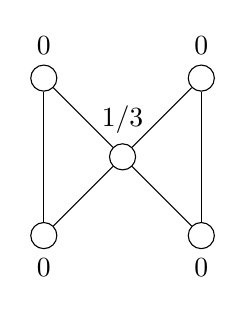
\begin{tikzpicture}
        \tikzstyle{vertex}=[circle, draw]
        \node[vertex, label=above:$1/3$](v) at (0, 0) {};
        \node[vertex, label=above:$0$](a) at (-1, 1) {};
        \node[vertex, label=above:$0$](b) at (1, 1) {};
        \node[vertex, label=below:$0$](c) at (-1,-1) {};
        \node[vertex, label=below:$0$](d) at (1,-1) {};
            \begin{scope}[every path/.style={-}, every node/.style={inner sep=1pt}]
                   \draw (a) -- (c);
                   \draw (b) -- (d);
                   \draw (a) -- (v);
                   \draw (b) -- (v);
                   \draw (c) -- (v);
                   \draw (d) -- (v);
            \end{scope} 
        \end{tikzpicture}
        \caption{The unique extreme point in the weak density polyhedron along the all-ones objective direction for the butterfly graph is as shown. The largest coordinate is $1/3$ and all other coordinates are $0$. Consequently, the integrality gap of the LP $\min\{\sum_{u\in V}x_u: x\in \weakdensitypolyhedron(G)\}$ is at least $3$.}
        \label{fig:butterfly-WD-integrality-gap}
     \end{subfigure}
     \hfill
     \begin{subfigure}[b]{0.47\textwidth}
    \centering
    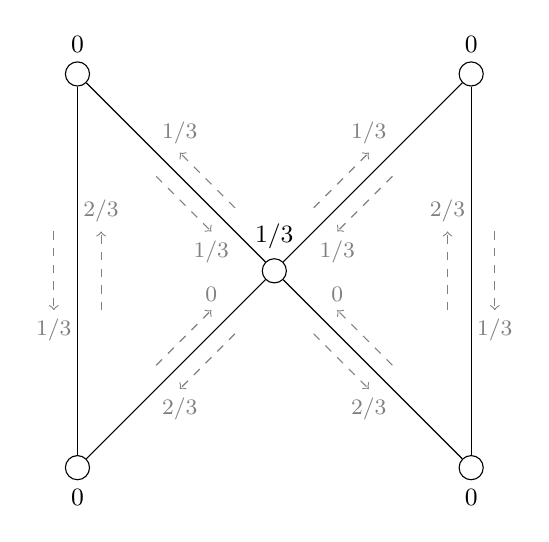
\begin{tikzpicture}
    \small
        \tikzstyle{vertex}=[circle, draw]
        \node[vertex, label=above:$1/3$](v) at (0, 0) {};
        \node[vertex, label=above:$0$](a) at (-2.5, 2.5) {};
        \node[vertex, label=above:$0$](b) at (2.5, 2.5) {};
        \node[vertex, label=below:$0$](c) at (-2.5,-2.5) {};
        \node[vertex, label=below:$0$](d) at (2.5,-2.5) {};
            % \begin{scope}[every path/.style={-}, every node/.style={inner sep=1pt}]
                    \draw (a) -- (c);
                   \draw (b) -- (d);
                   \draw (a) -- (v);
                   \draw (b) -- (v);
                   \draw (c) -- (v);
                   \draw (d) -- (v);
            % \end{scope} 

        \draw[->, gray, dashed] (-2.2, -0.5) to (-2.2, 0.5)  node[above] {\footnotesize $2/3$};
        \draw[->, gray, dashed] (-2.8, 0.5) to (-2.8, -0.5) node[below] {\footnotesize $1/3$};

        \draw[->, gray, dashed] (2.2, -0.5) to (2.2, 0.5) node[above] {\footnotesize $2/3$};
        \draw[->, gray, dashed] (2.8, 0.5) to (2.8, -0.5) node[below] {\footnotesize $1/3$};

        \draw[->, gray, dashed] (-1.5, -1.2) to (-0.8, -0.5) node[above] {\footnotesize $0$};
        \draw[->, gray, dashed] (-0.5, -0.8) to (-1.2, -1.5) node[below] {\footnotesize $2/3$};

        \draw[->, gray, dashed] (1.5, 1.2) to (0.8, 0.5) node[below] {\footnotesize $1/3$};
        \draw[->, gray, dashed] (0.5, 0.8) to (1.2, 1.5) node[above] {\footnotesize $1/3$};

        \draw[->, gray, dashed] (-1.5, 1.2) to (-0.8, 0.5) node[below] {\footnotesize $1/3$};
        \draw[->, gray, dashed] (-0.5, 0.8) to (-1.2, 1.5) node[above] {\footnotesize $1/3$};

        \draw[->, gray, dashed] (1.5, -1.2) to (0.8, -0.5) node[above] {\footnotesize $0$};
        \draw[->, gray, dashed] (0.5, -0.8) to (1.2, -1.5) node[below] {\footnotesize $2/3$};
        
        \end{tikzpicture}
        \caption{A minimal extreme point in the orientation polyhedron along the all-ones objective direction for the butterfly graph is as shown. The largest $x$-coordinate is $1/3$ and all other $x$-coordinates are $0$. Consequently, the integrality gap of the LP $\min\{\sum_{u\in V}x_u: x\in \orientationpolyhedron(G)\}$ is at least $3$.}
        \label{fig:butterfly-orientation-integrality-gap}
\end{subfigure}
     
\end{figure}


 
We emphasize that the extreme point result given in \Cref{thm:weak-density-extreme-point} and the integrality gap result mentioned in Corollary \ref{cor:thm:integrality-gap-3-WD-PFD} are interesting only from a polyhedral viewpoint currently, and are not of help from the perspective of algorithm design. This is because, implementing the above-mentioned iterative rounding procedure requires us to solve the LP-relaxation (\ref{PFDS-LP: WD}) in polynomial time, but we do not know how to do this yet. 

We next show that although $\projectedorientationpolyhedron(G)$ is a subset of $\weakdensitypolyhedron(G)$ (as shown in \Cref{lemma:orientation-formulation}), the extreme point result for $\weakdensitypolyhedron(G)$ given in \Cref{thm:weak-density-extreme-point} still holds for $\projectedorientationpolyhedron(G)$. We will say that an extreme point of a polyhedron is \emph{minimal} if for each variable, reducing the value of that variable by any $\epsilon>0$ while keeping the rest of the variables unchanged results in a point that is outside the polyhedron. We note that extreme points of a polyhedron along non-negative objective directions will be minimal. 

\begin{restatable}{theorem}{thmOrientationPolyhedronExtremePoint}
%\begin{theorem}
\label{thm:orientation-polyhedron-extreme-point}
Let $G=(V, E)$ be a graph that is not a pseudoforest. For every minimal extreme point $(x,y)$ of the polyhedron $\orientationpolyhedron(G)$, there exists a vertex $u\in V$ such that $x_u\ge 1/3$. 
%\end{theorem}
\end{restatable}

Similar to \Cref{cor:thm:integrality-gap-3-WD-PFD} that follows from \Cref{thm:weak-density-extreme-point}, \Cref{thm:orientation-polyhedron-extreme-point} implies the corollary below regarding the following LP-relaxation of \eqref{PFDS-IP:orient}: 
\begin{align}
    \min\left\{\sum \nolimits_{u\in V}c_u x_u: x\in \projectedorientationpolyhedron(G)\right\} \tag{PFDS-LP: orient} \label{PFDS-LP:orient}
\end{align}

\begin{thmcorollary}\label{cor:thm:integrality-gap-3-orientation}
The integrality gap of (\ref{PFDS-LP:orient}) is at most $3$. 
Moreover, given an extreme point optimum solution $x$ for the LP, there exists a polynomial time algorithm to obtain an integral feasible solution $x'$ for the LP-relaxation such that $\sum_{u\in V}c_u x'_u \le 3 \sum_{u\in V}c_u x_u$. 
\end{thmcorollary}

\Cref{cor:thm:integrality-gap-3-orientation} can be seen to follow from \Cref{thm:orientation-polyhedron-extreme-point} by the iterative rounding technique, where we repeatedly apply the following two steps until the graph $G$ is a pseudoforest: (1) Compute an extreme point optimum solution $x$ of $\min\left\{\sum_{u\in V}c_u x_u: x\in \projectedorientationpolyhedron(G)\right\}$. (2) By \Cref{thm:orientation-polyhedron-extreme-point}, there exists a vertex $u\in V$ such that $x_u\ge 1/3$; include the vertex $u$ in the solution and remove it from the graph $G$. The approximation factor of this procedure is $3$. In contrast to the weak density constraints based LP, namely (\ref{PFDS-LP: WD}), we can solve the orientation based LP, namely (\ref{PFDS-LP:orient}), in polynomial time. The example given in \Cref{fig:butterfly-orientation-integrality-gap} shows that the $(1/3)$-factor in \Cref{thm:orientation-polyhedron-extreme-point} and the integrality gap of $3$ mentioned in \Cref{cor:thm:integrality-gap-3-orientation} are both tight. 


\paragraph{FVS: poly-sized ILP formulations and LP integrality gaps.}
Next, we answer Question \ref{q:intro} affirmatively via a new ILP for FVS. 
In order to achieve this goal, we formulate an intermediate ILP for FVS whose
LP-relaxation has integrality gap at most $2$, but it is unclear if
this LP-relaxation is polynomial-time solvable.  We will later
formulate a \emph{polynomial-sized} ILP for FVS whose LP-relaxation is
at least as strong as that of the intermediate ILP, thereby achieving
our goal. Our intermediate ILP is based on weak density constraints and the following polyhedron that will be referred to as the cycle cover polyhedron: 
\begin{align}
\cyclecoverpolyhedron(G)&:=\left\{x\in \R^V_{\ge 0}: \sum \nolimits_{u\in U}x_u \ge 1 \ \forall U\subseteq V \text{ such that $G[U]$ contains a cycle}\right\}. \label{eqn:cycle-cover}
\end{align}
We will denote the constraints describing the cycle cover polyhedron as cycle cover constraints. 
It is known that the integrality gap of this polyhedron for FVS is $\Theta(\log n)$ \cite{BarYehudaGNR98}.
%\chandra{Added this fact which may not be obvious to the reader.}

For non-negative costs $c: V\rightarrow \R_{\ge 0}$, we consider the following formulation and its LP-relaxation:
\begin{align}
\min & \left\{\sum \nolimits_{u\in V}c_u x_u: x\in \weakdensitypolyhedron(G)\cap \cyclecoverpolyhedron(G)\cap \Z^V\right\} \quad \text{and} \tag{FVS-IP: WD-and-cycle-cover} \label{FVS-IP: WD-and-cycle-cover}\\
\min & \left\{\sum \nolimits_{u\in V} c_u x_u: x\in \weakdensitypolyhedron(G)\cap \cyclecoverpolyhedron(G)\right\}. \tag{FVS-LP: WD-and-cycle-cover}
\label{FVS-LP:weak-density-cycle-cover}
\end{align}


%\commentop{Chandra: Same comment about stating formulations inside theorem statements. The LP relaxation is just dropping the integrality constraint so having it repeated, especially inside a theorem statement is a bit odd to me.}
\begin{restatable}{theorem}{thmWeakDensityCycleCover}
%\begin{theorem}
\label{thm:integrality-gap-wd+cycle-cover}
For an input graph $G=(V, E)$ with non-negative costs $c: V\rightarrow \R_{\ge 0}$, \eqref{FVS-IP: WD-and-cycle-cover} is an integer linear programming formulation for FVS.  
Moreover, the integrality gap of \eqref{FVS-LP:weak-density-cycle-cover} is at most $2$. 
%Moreover, we have the following properties: 
% \begin{enumerate}
%     \item The integrality gap of the following LP-relaxation is at most $2$: 
% \begin{align*}
% \min\left\{\sum \nolimits_{u\in V} c_u x_u: x\in \weakdensitypolyhedron(G)\cap \cyclecoverpolyhedron(G)\right\}. \tag{FVS-LP: WD-and-cycle-cover}
% \label{FVS-LP:weak-density-cycle-cover}
% \end{align*}
%     \item There exists a polynomial-sized formulation for $\cyclecoverpolyhedron(G)$.  
% \end{enumerate}
%\end{theorem}
\end{restatable}
\Cref{thm:integrality-gap-wd+cycle-cover} shows that (\ref{FVS-IP: WD-and-cycle-cover}) is an ILP for FVS whose LP-relaxation (\ref{FVS-LP:weak-density-cycle-cover}) has integrality gap at most $2$. However, we do not have a polynomial-time algorithm to solve the LP-relaxation (\ref{FVS-LP:weak-density-cycle-cover}). This is because, we do not have a polynomial-time separation oracle for the family of weak density constraints (although we do have a polynomial-time separation oracle for the family of cycle cover constraints). 

\begin{remark}
In the spirit of using iterative rounding to bound integrality gaps (e.g., \Cref{thm:weak-density-extreme-point} that leads to \Cref{cor:thm:integrality-gap-3-WD-PFD} and \Cref{thm:orientation-polyhedron-extreme-point} that leads to \Cref{cor:thm:integrality-gap-3-orientation}), it is tempting to bound the integrality gap of (\ref{FVS-LP:weak-density-cycle-cover}) by proving an extreme point result. In particular, if we could show that every extreme point optimum of (\ref{FVS-LP:weak-density-cycle-cover}) had a coordinate with value at least $1/2$, then we would have an alternative proof of the integrality gap bound mentioned in \Cref{thm:integrality-gap-wd+cycle-cover} via the  iterative rounding technique. However, the example given in \Cref{fig:K4-WD-CC-integrality-gap} shows that there exists an extreme point optimum of (\ref{FVS-LP:weak-density-cycle-cover}) all of whose coordinates have value at most $1/3$. 
\end{remark} 



\begin{figure}[]
    % \centering
    % \begin{tikzpicture}
    %     \tikzstyle{vertex}=[circle, draw]
    %     \node[vertex, label=above:$1/3$](v) at (0, 0) {};
    %     \node[vertex, label=above:$0$](a) at (-2.5, 2.5) {};
    %     \node[vertex, label=above:$0$](b) at (2.5, 2.5) {};
    %     \node[vertex, label=below:$0$](c) at (-2.5,-2.5) {};
    %     \node[vertex, label=below:$0$](d) at (2.5,-2.5) {};
    %         % \begin{scope}[every path/.style={-}, every node/.style={inner sep=1pt}]
    %                 \draw (a) -- (c);
    %                \draw (b) -- (d);
    %                \draw (a) -- (v);
    %                \draw (b) -- (v);
    %                \draw (c) -- (v);
    %                \draw (d) -- (v);
    %         % \end{scope} 

    %     \draw[->, gray, dashed] (-2.2, -0.5) to (-2.2, 0.5)  node[above] {\footnotesize $2/3$};
    %     \draw[->, gray, dashed] (-2.8, 0.5) to (-2.8, -0.5) node[below] {\footnotesize $1/3$};

    %     \draw[->, gray, dashed] (2.2, -0.5) to (2.2, 0.5) node[above] {\footnotesize $2/3$};
    %     \draw[->, gray, dashed] (2.8, 0.5) to (2.8, -0.5) node[below] {\footnotesize $1/3$};

    %     \draw[->, gray, dashed] (-1.5, -1.2) to (-0.8, -0.5) node[above] {\footnotesize $0$};
    %     \draw[->, gray, dashed] (-0.5, -0.8) to (-1.2, -1.5) node[below] {\footnotesize $2/3$};

    %     \draw[->, gray, dashed] (1.5, 1.2) to (0.8, 0.5) node[below] {\footnotesize $1/3$};
    %     \draw[->, gray, dashed] (0.5, 0.8) to (1.2, 1.5) node[above] {\footnotesize $1/3$};

    %     \draw[->, gray, dashed] (-1.5, 1.2) to (-0.8, 0.5) node[below] {\footnotesize $1/3$};
    %     \draw[->, gray, dashed] (-0.5, 0.8) to (-1.2, 1.5) node[above] {\footnotesize $1/3$};

    %     \draw[->, gray, dashed] (1.5, -1.2) to (0.8, -0.5) node[above] {\footnotesize $0$};
    %     \draw[->, gray, dashed] (0.5, -0.8) to (1.2, -1.5) node[below] {\footnotesize $2/3$};
        
    %     \end{tikzpicture}
    %     \caption{An extreme point of the butterfly graph in the orientation polyhedron along all-ones objective direction is as shown. The largest $x$-coordinate is $1/3$ and all other $x$-coordinates are $0$. Consequently, the integrality gap of the LP $\max\{\sum_{u\in V}x_u: x\in \orientationpolyhedron(G)\}$ is at least $3$.}
    %     \label{fig:butterfly-orientation-integrality-gap}
    
     \centering
    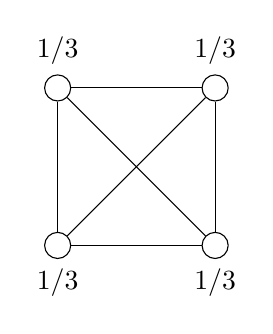
\begin{tikzpicture}
        \tikzstyle{vertex}=[circle, draw]
        % \node[vertex, label=above:$1/3$](v) at (0, 0) {$v$};
        \node[vertex, label=above:$1/3$](a) at (-1, 1) {};
        \node[vertex, label=above:$1/3$](b) at (1, 1) {};
        \node[vertex, label=below:$1/3$](c) at (-1,-1) {};
        \node[vertex, label=below:$1/3$](d) at (1,-1) {};
            \begin{scope}[every path/.style={-}, every node/.style={inner sep=1pt}]
                   \draw (a) -- (b);
                   \draw (a) -- (c);
                   \draw (a) -- (d);
                   \draw (b) -- (c);
                   \draw (b) -- (d);
                   \draw (c) -- (d);
            \end{scope} 
        \end{tikzpicture}
        \caption{The unique extreme point optimum for (\ref{FVS-LP:weak-density-cycle-cover}) along the all-ones objective direction on the complete graph $K_4$ is as shown. Consequently, the integrality gap of (\ref{FVS-LP:weak-density-cycle-cover}) is at least $3$.}
        \label{fig:K4-WD-CC-integrality-gap}
\end{figure}

We will use \Cref{lemma:orientation-formulation} in conjunction with \Cref{thm:integrality-gap-wd+cycle-cover} to prove the following result: 
\begin{theorem}\label{thm:poly-sized-LP-with-integrality-gap-atmost-2-for-FVS} 
There exists a polynomial-sized integer linear programming formulation for FVS whose LP-relaxation has integrality gap at most $2$. 
\end{theorem}
We prove \Cref{thm:poly-sized-LP-with-integrality-gap-atmost-2-for-FVS} by showing three different polynomial-sized integer linear programs for FVS all of whose LP-relaxations have integrality gap at most $2$:
\begin{enumerate}
\item The first formulation is 
\begin{align*}
    \min\left\{\sum \nolimits_{u\in V}c_u x_u: x\in \projectedorientationpolyhedron(G)\cap \cyclecoverpolyhedron(G)\cap \Z^V\right\}. \tag{FVS-IP: orient-and-cycle-cover} %\label{FVS-IP: orient-and-cycle-cover}
\end{align*}
%$\min\{\sum_{u\in V}c_u x_u: x\in \projectedorientationpolyhedron(G)\cap \cyclecoverpolyhedron(G)\cap \Z^V\}$. 
By \Cref{lemma:orientation-formulation}(1), we have that  $\projectedorientationpolyhedron(G)\subseteq \weakdensitypolyhedron(G)$. As a consequence of \Cref{thm:integrality-gap-wd+cycle-cover}, the integrality gap of the following LP-relaxation is also at most $2$: 
\begin{align}
    \min\left\{\sum \nolimits_{u\in V}c_u x_u: x\in \projectedorientationpolyhedron(G)\cap \cyclecoverpolyhedron(G)\right\}.  \tag{FVS-LP: orient-and-cycle-cover} \label{FVS-LP: orient-and-cycle-cover}
\end{align}
%$\min\{\sum_{u\in V}c_u x_u: x\in \projectedorientationpolyhedron(G)\cap \cyclecoverpolyhedron(G)\}$ 
Both $\projectedorientationpolyhedron(G)$ and $\cyclecoverpolyhedron(G)$ admit a polynomial-sized description (see \Cref{lemma:cycle-cover-poly-sized-lp} in \Cref{sec:cycle-cover-poly-sized-formulation} for polynomial-sized description of $\cyclecoverpolyhedron(G)$), and thus, we have a polynomial-sized ILP for FVS whose LP-relaxation has integrality gap at most $2$.

\item The second formulation is the Chekuri-Madan formulation who, as
  we remarked earlier, formulated an ILP for Subset-FVS and showed
  that the integrality gap of its LP-relaxation is at most $13$
  \cite{chekuri-madan16}. We show that
  their LP-relaxation specialized for FVS has integrality gap at most
  $2$ by proving that it is at least as strong as
%the LP-relaxation of our first formulation, i.e., 
  (\ref{FVS-LP: orient-and-cycle-cover}). Our result gives additional impetus
  to improving the integrality gap of their LP-relaxation for Subset-FVS. 

\item Our third formulation to prove \Cref{thm:poly-sized-LP-with-integrality-gap-atmost-2-for-FVS} is based on the orientation perspective, but without cycle cover constraints (as opposed to our first formulation). Here, we give an orientation based ILP formulation whose associated polyhedron is contained in the strong density polyhedron. Since the integrality gap of (\ref{FVS-LP: SD}) is at most $2$ (as shown by Chudak, Goemans, Hochbaum, and Williamson \cite{CHUDAK1998111}), the integrality gap of our third formulation is also at most $2$.   
\end{enumerate}

We emphasize that the proof of the integrality gap of the
LP-relaxation of all three of our ILPs rely on the integrality gap
upper bound of (\ref{FVS-LP:weak-density-cycle-cover}) or (\ref{FVS-LP:
  SD}). It would be interesting to have a direct proof. In particular,
it would be useful to design a primal rounding algorithm (for arbitrary
LP-optimum solutions or for extreme point LP-optimum solutions) that
yields a $2$-approximate solution.


%We present formal statements of our results in this section. 
% We recall that our main goal is to formulate an integer linear program
% (ILP) for FVS whose LP-relaxation has integrality gap at most $2$. As
% our first result, we show how to achieve this goal for PFDS by giving
% a new ILP formulation. We will subsequently use the properties of our
% new ILP formulation for PFDS to achieve the goal for FVS.





\paragraph{Organization.} 
We focus on PFDS in Section 3 and FVS in Section 4. In Section \ref{sec:orientatin-polytope}, we prove properties of the orientation polyhedron and show \Cref{lemma:orientation-formulation}. 
In Sections \ref{sec:extreme-point-weak-density} and \ref{sec:orientation-polytope-extreme-point}, we prove extreme point properties of the weak density polyhedron and the orientation polyhedron and show Theorems \ref{thm:weak-density-extreme-point} and \ref{thm:orientation-polyhedron-extreme-point} respectively. 
In Section \ref{sec:integrality-gap-of-weak-density-and-cycle-cover}, we prove properties of the weak density polyhedron and 
%, show that the cycle cover polyhedron admits a polynomial-sized formulation, and 
show \Cref{thm:integrality-gap-wd+cycle-cover}. 
In Section \ref{sec:orientation-and-cycle-cover-formulation}, we give a polynomial-sized ILP formulation for FVS with integrality gap at most $2$, thereby proving \Cref{thm:poly-sized-LP-with-integrality-gap-atmost-2-for-FVS}. For the sake of completeness, we discuss two additional polynomial-sized ILP formulations for FVS with integrality gap at most $2$ in Section \ref{sec:more-FVS-formulations}. 

\iffalse
In Section \ref{sec:orientatin-polytope}, we prove properties of the orientation polyhedron and show \Cref{lemma:orientation-formulation}. 
In Section \ref{sec:integrality-gap-of-weak-density-and-cycle-cover}, we prove properties of the weak density polyhedron and 
%, show that the cycle cover polyhedron admits a polynomial-sized formulation, and 
show \Cref{thm:integrality-gap-wd+cycle-cover}. 
In Section \ref{sec:poly-sized-lp-relaxation-with-gap-atmost-two-for-fvs}, we show three different polynomial-sized ILPs for FVS whose LP-relaxation has integrality gap at most $2$, thereby proving \Cref{thm:poly-sized-LP-with-integrality-gap-atmost-2-for-FVS}. In Sections \ref{sec:extreme-point-weak-density} and \ref{sec:orientation-polytope-extreme-point}, we prove extreme point properties of the weak density polyhedron and the orientation polyhedron and show \Cref{thm:weak-density-extreme-point} and \Cref{thm:orientation-polyhedron-extreme-point} respectively. 
\fi